\section{Background and Motivation}
\subsection{Workloads}
\ VGGNet:VGGNet is a deep convolutional neural network developed by the Computer Vision Group at Oxford University and researchers at Google DeepMind. VGGNet explores the relationship between the depth of a convolutional neural network and its performance. By repeatedly stacking 3*3 small convolutional kernels and 2*2 largest pooled layers, VGGNet successfully builds a 16-19 layer deep convolution.\cite{simonyan2014very} Neural Networks. Compared with the previous network structure, VGGNet significantly reduced the error rate, and achieved the second place of the ILSVRC 2014 competition classification project and the first place of the positioning project. At the same time, VGGNet's scalability is very strong, and the generalization performance of migrating to other image data is very good. VGGNet's structure is very simple, the entire network uses the same size of the convolution kernel size and maximum pool size.So far, VGGNet is still often used to extract image features.


Inception Net: Google Inception Net won first place in the ILSVRC 2014 competition. The Inception Net in the game is usually called Inception V1. Its greatest feature is that it controls the calculations and parameters while achieving very good classification performance. Inception V1 proposes Inception Module to increase the utilization of parameters. Although his depth reaches 22 levels, the parameter amount is much lower than ALexNet and VGGNet. Subsequently, Inception V2, Inception V3 and Inception V4 emerged successively in 2015 and 2016. Inception V2 refers to VGGNet and uses two 3*3 convolutions instead of a 5*5 convolution to reduce the amount of parameters. At the same time, the famous method of Batch Normalization was proposed to speed up the training of the network, and the accuracy of the classification after convergence can also be improved. Inception V3 splits the larger two-dimensional convolutional network into a smaller one-dimensional convolutional network. On the one hand, it saves a lot of parameters, speeds up calculations, and reduces over-fitting. It also adds a layer of non-linear expansion model. Ability to express so that the network can handle more and more abundant spatial features and increase the diversity of features. On the other hand, Inception V3 optimizes the structure of the Inception Module. Subsequent Inception V4 further integrated Resnet on the basis of Inception V3 to further improve accuracy.


Resnet: Microsoft Researcher Kaiming He and others proposed Resnet and won the championship in ILSVRC 2015. Resnet's TOP5 error rate was only 3.75\%.Resnet uses a connection method called "shortcut connection" to reduce network parameters, and stack the input and output of the block. This simple addition will not add extra parameters and calculations to the network, but it can greatly increase the training speed of the model, improve the training effect, and when the number of layers of the model deepens, this simple structure can solve the problem of degradation well. There are two different learning units in Resnet's structure: two levels of residual learning units and three levels of residual learning units. The two-level residual learning unit contains two 3*3 convolutions with the same number of output channels. The three-level residual network uses a 1*1 convolution before and after the middle 3*3 convolution. The 50,101,152-layer networks we use are mainly three-tier residual structures.


MobileNet: MobileNet was proposed by Horward et al. in 2017. Its architecture consists of a standard convolution layer acting on the input image, a deep separable convolutional stack, and a final average pool and fully connected layer. Mobilenet uses a deeply separable convolution to build a lightweight, deep neural network that can integrate standard volumes into a deep convolution and a dot convolution (1 × 1 convolution kernel). Depth convolution applies each convolution kernel to each channel, and 1 × 1 convolution is used to combine the output of channel convolutions. This decomposition can effectively reduce the computation and reduce the model size. MobileNet has a clear advantage in terms of computational volume and model size.

\subsection{Motivation}
\ref{fig:motivation}

\begin{figure}[!t]
\centering
\subfloat[][Model size]{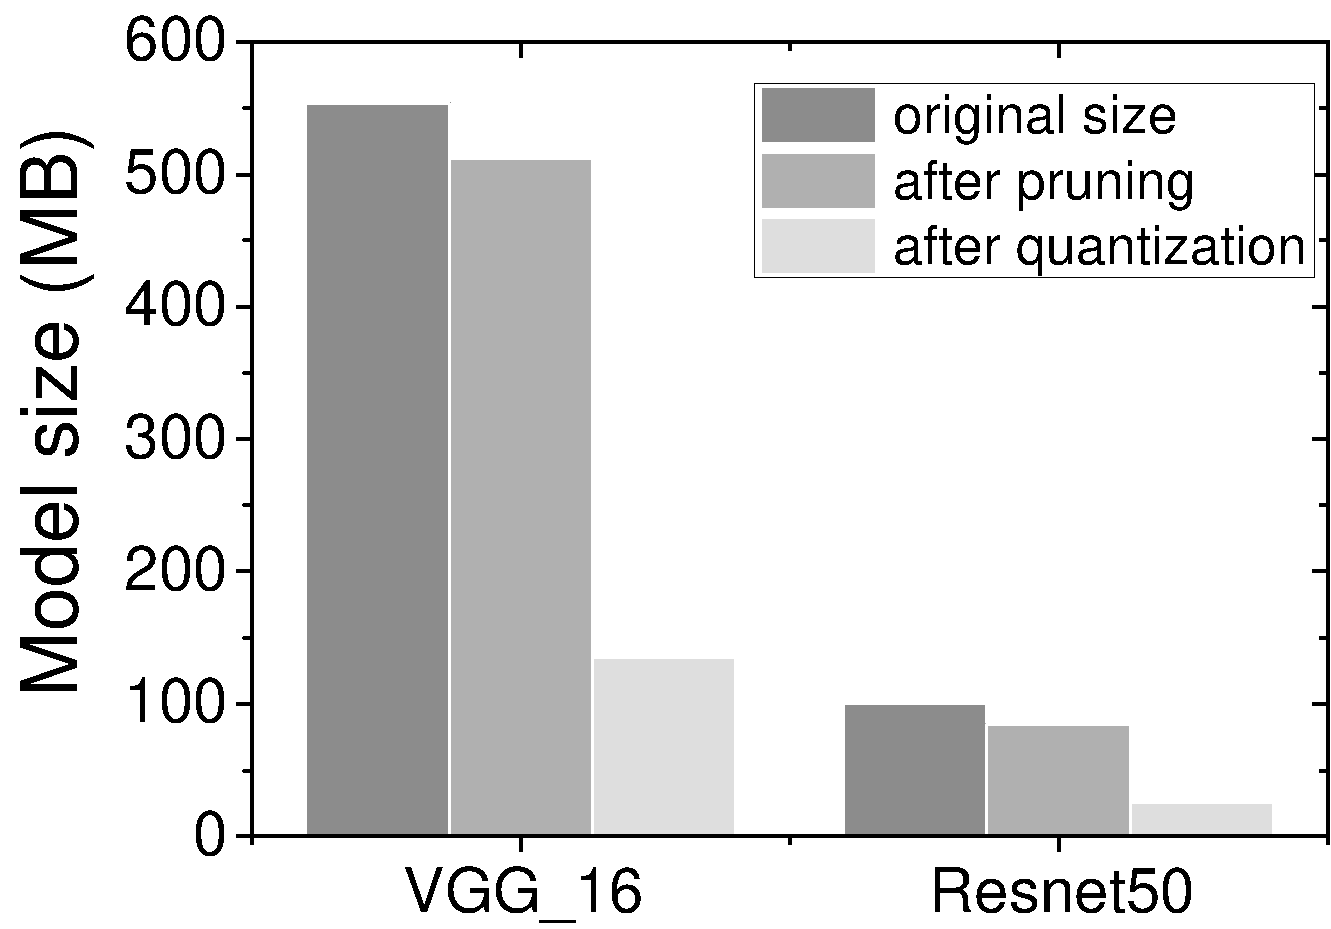
\includegraphics[width=0.4\textwidth]{figure/motivation_size.pdf}}
\hfill
\subfloat[][Inference time]{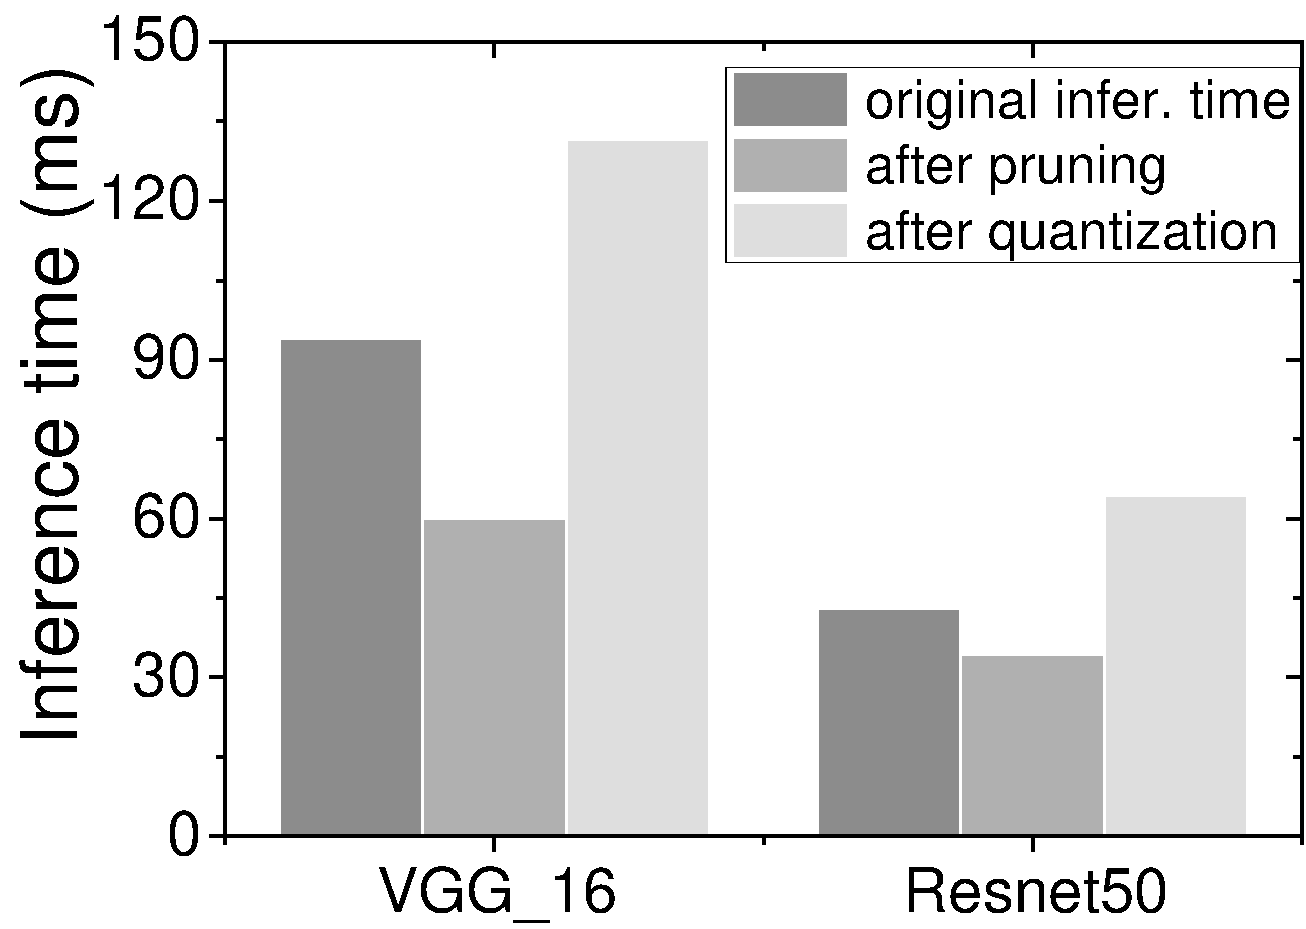
\includegraphics[width=0.4\textwidth]{figure/motivation_time.pdf}}
\caption{The achieved model size (a) and inference time (b) before and after the compression by quantization and pruning.
There is significant room for improvement.} 
\label{fig:motivation}
\end{figure}